\documentclass[twoside]{book}

% Packages required by doxygen
\usepackage{fixltx2e}
\usepackage{calc}
\usepackage{doxygen}
\usepackage[export]{adjustbox} % also loads graphicx
\usepackage{graphicx}
\usepackage[utf8]{inputenc}
\usepackage{makeidx}
\usepackage{multicol}
\usepackage{multirow}
\PassOptionsToPackage{warn}{textcomp}
\usepackage{textcomp}
\usepackage[nointegrals]{wasysym}
\usepackage[table]{xcolor}

% Font selection
\usepackage[T1]{fontenc}
\usepackage[scaled=.90]{helvet}
\usepackage{courier}
\usepackage{amssymb}
\usepackage{sectsty}
\renewcommand{\familydefault}{\sfdefault}
\allsectionsfont{%
  \fontseries{bc}\selectfont%
  \color{darkgray}%
}
\renewcommand{\DoxyLabelFont}{%
  \fontseries{bc}\selectfont%
  \color{darkgray}%
}
\newcommand{\+}{\discretionary{\mbox{\scriptsize$\hookleftarrow$}}{}{}}

% Page & text layout
\usepackage{geometry}
\geometry{%
  a4paper,%
  top=2.5cm,%
  bottom=2.5cm,%
  left=2.5cm,%
  right=2.5cm%
}
\tolerance=750
\hfuzz=15pt
\hbadness=750
\setlength{\emergencystretch}{15pt}
\setlength{\parindent}{0cm}
\setlength{\parskip}{3ex plus 2ex minus 2ex}
\makeatletter
\renewcommand{\paragraph}{%
  \@startsection{paragraph}{4}{0ex}{-1.0ex}{1.0ex}{%
    \normalfont\normalsize\bfseries\SS@parafont%
  }%
}
\renewcommand{\subparagraph}{%
  \@startsection{subparagraph}{5}{0ex}{-1.0ex}{1.0ex}{%
    \normalfont\normalsize\bfseries\SS@subparafont%
  }%
}
\makeatother

% Headers & footers
\usepackage{fancyhdr}
\pagestyle{fancyplain}
\fancyhead[LE]{\fancyplain{}{\bfseries\thepage}}
\fancyhead[CE]{\fancyplain{}{}}
\fancyhead[RE]{\fancyplain{}{\bfseries\leftmark}}
\fancyhead[LO]{\fancyplain{}{\bfseries\rightmark}}
\fancyhead[CO]{\fancyplain{}{}}
\fancyhead[RO]{\fancyplain{}{\bfseries\thepage}}
\fancyfoot[LE]{\fancyplain{}{}}
\fancyfoot[CE]{\fancyplain{}{}}
\fancyfoot[RE]{\fancyplain{}{\bfseries\scriptsize Generated by Doxygen }}
\fancyfoot[LO]{\fancyplain{}{\bfseries\scriptsize Generated by Doxygen }}
\fancyfoot[CO]{\fancyplain{}{}}
\fancyfoot[RO]{\fancyplain{}{}}
\renewcommand{\footrulewidth}{0.4pt}
\renewcommand{\chaptermark}[1]{%
  \markboth{#1}{}%
}
\renewcommand{\sectionmark}[1]{%
  \markright{\thesection\ #1}%
}

% Indices & bibliography
\usepackage{natbib}
\usepackage[titles]{tocloft}
\setcounter{tocdepth}{3}
\setcounter{secnumdepth}{5}
\makeindex

% Hyperlinks (required, but should be loaded last)
\usepackage{ifpdf}
\ifpdf
  \usepackage[pdftex,pagebackref=true]{hyperref}
\else
  \usepackage[ps2pdf,pagebackref=true]{hyperref}
\fi
\hypersetup{%
  colorlinks=true,%
  linkcolor=blue,%
  citecolor=blue,%
  unicode%
}

% Custom commands
\newcommand{\clearemptydoublepage}{%
  \newpage{\pagestyle{empty}\cleardoublepage}%
}

\usepackage{caption}
\captionsetup{labelsep=space,justification=centering,font={bf},singlelinecheck=off,skip=4pt,position=top}

%===== C O N T E N T S =====

\begin{document}

% Titlepage & ToC
\hypersetup{pageanchor=false,
             bookmarksnumbered=true,
             pdfencoding=unicode
            }
\pagenumbering{alph}
\begin{titlepage}
\vspace*{7cm}
\begin{center}%
{\Large Dungeons and Dragons Manager \\[1ex]\large 1.\+0 }\\
\vspace*{1cm}
{\large Generated by Doxygen 1.8.14}\\
\end{center}
\end{titlepage}
\clearemptydoublepage
\pagenumbering{roman}
\tableofcontents
\clearemptydoublepage
\pagenumbering{arabic}
\hypersetup{pageanchor=true}

%--- Begin generated contents ---
\chapter{Namespace Index}
\section{Namespace List}
Here is a list of all documented namespaces with brief descriptions\+:\begin{DoxyCompactList}
\item\contentsline{section}{\mbox{\hyperlink{namespace_dungeons__n___dragons___manager}{Dungeons\+\_\+n\+\_\+\+Dragons\+\_\+\+Manager}} }{\pageref{namespace_dungeons__n___dragons___manager}}{}
\item\contentsline{section}{\mbox{\hyperlink{namespace_dungeons__n___dragons___manager_1_1_controls}{Dungeons\+\_\+n\+\_\+\+Dragons\+\_\+\+Manager.\+Controls}} }{\pageref{namespace_dungeons__n___dragons___manager_1_1_controls}}{}
\item\contentsline{section}{\mbox{\hyperlink{namespace_dungeons__n___dragons___manager_1_1_models}{Dungeons\+\_\+n\+\_\+\+Dragons\+\_\+\+Manager.\+Models}} }{\pageref{namespace_dungeons__n___dragons___manager_1_1_models}}{}
\item\contentsline{section}{\mbox{\hyperlink{namespace_dungeons__n___dragons___manager_1_1_tools}{Dungeons\+\_\+n\+\_\+\+Dragons\+\_\+\+Manager.\+Tools}} }{\pageref{namespace_dungeons__n___dragons___manager_1_1_tools}}{}
\item\contentsline{section}{\mbox{\hyperlink{namespace_dungeons__n___dragons___manager_1_1_viewmodels}{Dungeons\+\_\+n\+\_\+\+Dragons\+\_\+\+Manager.\+Viewmodels}} }{\pageref{namespace_dungeons__n___dragons___manager_1_1_viewmodels}}{}
\item\contentsline{section}{\mbox{\hyperlink{namespace_dungeons__n___dragons___manager_1_1_windows}{Dungeons\+\_\+n\+\_\+\+Dragons\+\_\+\+Manager.\+Windows}} }{\pageref{namespace_dungeons__n___dragons___manager_1_1_windows}}{}
\end{DoxyCompactList}

\chapter{Hierarchical Index}
\section{Class Hierarchy}
This inheritance list is sorted roughly, but not completely, alphabetically\+:\begin{DoxyCompactList}
\item \contentsline{section}{Dungeons\+\_\+n\+\_\+\+Dragons\+\_\+\+Manager.\+Models.\+Character}{\pageref{class_dungeons__n___dragons___manager_1_1_models_1_1_character}}{}
\item \contentsline{section}{Dungeons\+\_\+n\+\_\+\+Dragons\+\_\+\+Manager.\+Viewmodels.\+Characters\+Tab\+Viewmodel}{\pageref{class_dungeons__n___dragons___manager_1_1_viewmodels_1_1_characters_tab_viewmodel}}{}
\item \contentsline{section}{Dungeons\+\_\+n\+\_\+\+Dragons\+\_\+\+Manager.\+Viewmodels.\+Create\+Character\+Window\+Viewmodel}{\pageref{class_dungeons__n___dragons___manager_1_1_viewmodels_1_1_create_character_window_viewmodel}}{}
\item I\+Command\begin{DoxyCompactList}
\item \contentsline{section}{Dungeons\+\_\+n\+\_\+\+Dragons\+\_\+\+Manager.\+Tools.\+Command\+Handler}{\pageref{class_dungeons__n___dragons___manager_1_1_tools_1_1_command_handler}}{}
\end{DoxyCompactList}
\item I\+Notify\+Property\+Changed\begin{DoxyCompactList}
\item \contentsline{section}{Dungeons\+\_\+n\+\_\+\+Dragons\+\_\+\+Manager.\+Models.\+Dice\+Bag}{\pageref{class_dungeons__n___dragons___manager_1_1_models_1_1_dice_bag}}{}
\item \contentsline{section}{Dungeons\+\_\+n\+\_\+\+Dragons\+\_\+\+Manager.\+Viewmodels.\+Dice\+Roll\+Tab\+Viewmodel}{\pageref{class_dungeons__n___dragons___manager_1_1_viewmodels_1_1_dice_roll_tab_viewmodel}}{}
\item \contentsline{section}{Dungeons\+\_\+n\+\_\+\+Dragons\+\_\+\+Manager.\+Viewmodels.\+Encounters\+Tab\+Viewmodel}{\pageref{class_dungeons__n___dragons___manager_1_1_viewmodels_1_1_encounters_tab_viewmodel}}{}
\end{DoxyCompactList}
\item \contentsline{section}{Dungeons\+\_\+n\+\_\+\+Dragons\+\_\+\+Manager.\+Viewmodels.\+Main\+Window\+Viewmodel}{\pageref{class_dungeons__n___dragons___manager_1_1_viewmodels_1_1_main_window_viewmodel}}{}
\item \contentsline{section}{Dungeons\+\_\+n\+\_\+\+Dragons\+\_\+\+Manager.\+Models.\+Monster}{\pageref{class_dungeons__n___dragons___manager_1_1_models_1_1_monster}}{}
\item User\+Control\begin{DoxyCompactList}
\item \contentsline{section}{Dungeons\+\_\+n\+\_\+\+Dragons\+\_\+\+Manager.\+Controls.\+Characters\+Tab\+Control}{\pageref{class_dungeons__n___dragons___manager_1_1_controls_1_1_characters_tab_control}}{}
\item \contentsline{section}{Dungeons\+\_\+n\+\_\+\+Dragons\+\_\+\+Manager.\+Controls.\+Dice\+Roll\+Tab\+Control}{\pageref{class_dungeons__n___dragons___manager_1_1_controls_1_1_dice_roll_tab_control}}{}
\item \contentsline{section}{Dungeons\+\_\+n\+\_\+\+Dragons\+\_\+\+Manager.\+Controls.\+Encounters\+Tab\+Control}{\pageref{class_dungeons__n___dragons___manager_1_1_controls_1_1_encounters_tab_control}}{}
\end{DoxyCompactList}
\item Window\begin{DoxyCompactList}
\item \contentsline{section}{Dungeons\+\_\+n\+\_\+\+Dragons\+\_\+\+Manager.\+Windows.\+Create\+Character\+Window}{\pageref{class_dungeons__n___dragons___manager_1_1_windows_1_1_create_character_window}}{}
\item \contentsline{section}{Dungeons\+\_\+n\+\_\+\+Dragons\+\_\+\+Manager.\+Windows.\+Main\+Window}{\pageref{class_dungeons__n___dragons___manager_1_1_windows_1_1_main_window}}{}
\end{DoxyCompactList}
\end{DoxyCompactList}

\chapter{Class Index}
\section{Class List}
Here are the classes, structs, unions and interfaces with brief descriptions\+:\begin{DoxyCompactList}
\item\contentsline{section}{\mbox{\hyperlink{class_dungeons__n___dragons___manager_1_1_models_1_1_character}{Dungeons\+\_\+n\+\_\+\+Dragons\+\_\+\+Manager.\+Models.\+Character}} \\*A model to hold character data. }{\pageref{class_dungeons__n___dragons___manager_1_1_models_1_1_character}}{}
\item\contentsline{section}{\mbox{\hyperlink{class_dungeons__n___dragons___manager_1_1_controls_1_1_characters_tab_control}{Dungeons\+\_\+n\+\_\+\+Dragons\+\_\+\+Manager.\+Controls.\+Characters\+Tab\+Control}} \\*Interaction logic for Characters\+Tab\+Control.\+xaml }{\pageref{class_dungeons__n___dragons___manager_1_1_controls_1_1_characters_tab_control}}{}
\item\contentsline{section}{\mbox{\hyperlink{class_dungeons__n___dragons___manager_1_1_viewmodels_1_1_characters_tab_viewmodel}{Dungeons\+\_\+n\+\_\+\+Dragons\+\_\+\+Manager.\+Viewmodels.\+Characters\+Tab\+Viewmodel}} \\*Viewmodel for the Characters Tab in the Main Window. }{\pageref{class_dungeons__n___dragons___manager_1_1_viewmodels_1_1_characters_tab_viewmodel}}{}
\item\contentsline{section}{\mbox{\hyperlink{class_dungeons__n___dragons___manager_1_1_tools_1_1_command_handler}{Dungeons\+\_\+n\+\_\+\+Dragons\+\_\+\+Manager.\+Tools.\+Command\+Handler}} \\*Class that handles the command routing. }{\pageref{class_dungeons__n___dragons___manager_1_1_tools_1_1_command_handler}}{}
\item\contentsline{section}{\mbox{\hyperlink{class_dungeons__n___dragons___manager_1_1_windows_1_1_create_character_window}{Dungeons\+\_\+n\+\_\+\+Dragons\+\_\+\+Manager.\+Windows.\+Create\+Character\+Window}} \\*Interaction logic for Create\+Character\+Window.\+xaml }{\pageref{class_dungeons__n___dragons___manager_1_1_windows_1_1_create_character_window}}{}
\item\contentsline{section}{\mbox{\hyperlink{class_dungeons__n___dragons___manager_1_1_viewmodels_1_1_create_character_window_viewmodel}{Dungeons\+\_\+n\+\_\+\+Dragons\+\_\+\+Manager.\+Viewmodels.\+Create\+Character\+Window\+Viewmodel}} \\*The viewmodel for creating characters }{\pageref{class_dungeons__n___dragons___manager_1_1_viewmodels_1_1_create_character_window_viewmodel}}{}
\item\contentsline{section}{\mbox{\hyperlink{class_dungeons__n___dragons___manager_1_1_models_1_1_dice_bag}{Dungeons\+\_\+n\+\_\+\+Dragons\+\_\+\+Manager.\+Models.\+Dice\+Bag}} \\*\mbox{\hyperlink{class_dungeons__n___dragons___manager_1_1_models_1_1_dice_bag}{Dice\+Bag}} class containing rolling functions dice enum. }{\pageref{class_dungeons__n___dragons___manager_1_1_models_1_1_dice_bag}}{}
\item\contentsline{section}{\mbox{\hyperlink{class_dungeons__n___dragons___manager_1_1_controls_1_1_dice_roll_tab_control}{Dungeons\+\_\+n\+\_\+\+Dragons\+\_\+\+Manager.\+Controls.\+Dice\+Roll\+Tab\+Control}} \\*Interaction logic for Dice\+Roll\+Tab\+Control.\+xaml }{\pageref{class_dungeons__n___dragons___manager_1_1_controls_1_1_dice_roll_tab_control}}{}
\item\contentsline{section}{\mbox{\hyperlink{class_dungeons__n___dragons___manager_1_1_viewmodels_1_1_dice_roll_tab_viewmodel}{Dungeons\+\_\+n\+\_\+\+Dragons\+\_\+\+Manager.\+Viewmodels.\+Dice\+Roll\+Tab\+Viewmodel}} \\*viewmodel for the roll dice tab }{\pageref{class_dungeons__n___dragons___manager_1_1_viewmodels_1_1_dice_roll_tab_viewmodel}}{}
\item\contentsline{section}{\mbox{\hyperlink{class_dungeons__n___dragons___manager_1_1_controls_1_1_encounters_tab_control}{Dungeons\+\_\+n\+\_\+\+Dragons\+\_\+\+Manager.\+Controls.\+Encounters\+Tab\+Control}} \\*Interaction logic for Encounters\+Tab\+Control.\+xaml }{\pageref{class_dungeons__n___dragons___manager_1_1_controls_1_1_encounters_tab_control}}{}
\item\contentsline{section}{\mbox{\hyperlink{class_dungeons__n___dragons___manager_1_1_viewmodels_1_1_encounters_tab_viewmodel}{Dungeons\+\_\+n\+\_\+\+Dragons\+\_\+\+Manager.\+Viewmodels.\+Encounters\+Tab\+Viewmodel}} \\*Viewmodel for the Encounters Tab in the Main Window. }{\pageref{class_dungeons__n___dragons___manager_1_1_viewmodels_1_1_encounters_tab_viewmodel}}{}
\item\contentsline{section}{\mbox{\hyperlink{class_dungeons__n___dragons___manager_1_1_windows_1_1_main_window}{Dungeons\+\_\+n\+\_\+\+Dragons\+\_\+\+Manager.\+Windows.\+Main\+Window}} \\*Interaction logic for Main\+Window.\+xaml }{\pageref{class_dungeons__n___dragons___manager_1_1_windows_1_1_main_window}}{}
\item\contentsline{section}{\mbox{\hyperlink{class_dungeons__n___dragons___manager_1_1_viewmodels_1_1_main_window_viewmodel}{Dungeons\+\_\+n\+\_\+\+Dragons\+\_\+\+Manager.\+Viewmodels.\+Main\+Window\+Viewmodel}} \\*Viewmodel for the main window. }{\pageref{class_dungeons__n___dragons___manager_1_1_viewmodels_1_1_main_window_viewmodel}}{}
\item\contentsline{section}{\mbox{\hyperlink{class_dungeons__n___dragons___manager_1_1_models_1_1_monster}{Dungeons\+\_\+n\+\_\+\+Dragons\+\_\+\+Manager.\+Models.\+Monster}} \\*A model to hold monster data. }{\pageref{class_dungeons__n___dragons___manager_1_1_models_1_1_monster}}{}
\end{DoxyCompactList}

\chapter{Namespace Documentation}
\hypertarget{namespace_dungeons__n___dragons___manager}{}\section{Dungeons\+\_\+n\+\_\+\+Dragons\+\_\+\+Manager Namespace Reference}
\label{namespace_dungeons__n___dragons___manager}\index{Dungeons\+\_\+n\+\_\+\+Dragons\+\_\+\+Manager@{Dungeons\+\_\+n\+\_\+\+Dragons\+\_\+\+Manager}}
\subsection*{Classes}
\begin{DoxyCompactItemize}
\item 
class \mbox{\hyperlink{class_dungeons__n___dragons___manager_1_1_app}{App}}
\begin{DoxyCompactList}\small\item\em Interaction logic for App.\+xaml \end{DoxyCompactList}\end{DoxyCompactItemize}

\chapter{Class Documentation}
\hypertarget{class_dungeons__n___dragons___manager_1_1_app}{}\section{Dungeons\+\_\+n\+\_\+\+Dragons\+\_\+\+Manager.\+App Class Reference}
\label{class_dungeons__n___dragons___manager_1_1_app}\index{Dungeons\+\_\+n\+\_\+\+Dragons\+\_\+\+Manager.\+App@{Dungeons\+\_\+n\+\_\+\+Dragons\+\_\+\+Manager.\+App}}


Interaction logic for App.\+xaml  


Inheritance diagram for Dungeons\+\_\+n\+\_\+\+Dragons\+\_\+\+Manager.\+App\+:\begin{figure}[H]
\begin{center}
\leavevmode
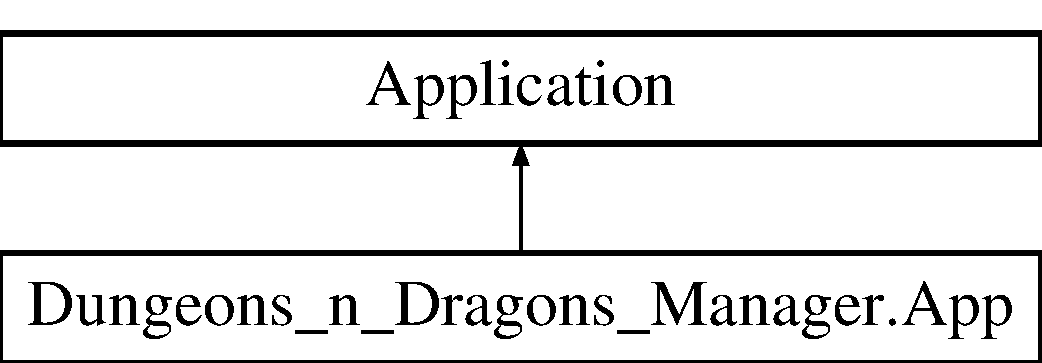
\includegraphics[height=2.000000cm]{class_dungeons__n___dragons___manager_1_1_app}
\end{center}
\end{figure}


\subsection{Detailed Description}
Interaction logic for App.\+xaml 



The documentation for this class was generated from the following file\+:\begin{DoxyCompactItemize}
\item 
C\+:/\+Users/\+Seth Peterson/\+Desktop/\+School/\+E\+E\+C\+S448/\+Project3/\+Dungeons\+\_\+n\+\_\+\+Dragons\+\_\+\+Manager/\+Dungeons\+\_\+n\+\_\+\+Dragons\+\_\+\+Manager/\+Dungeons\+\_\+n\+\_\+\+Dragons\+\_\+\+Manager/App.\+xaml.\+cs\end{DoxyCompactItemize}

%--- End generated contents ---

% Index
\backmatter
\newpage
\phantomsection
\clearemptydoublepage
\addcontentsline{toc}{chapter}{Index}
\printindex

\end{document}
